\documentclass[a4paper]{article}

\usepackage[T1]{fontenc}
\usepackage{lmodern}
\usepackage[utf8]{inputenc} 
\usepackage{graphicx}
\usepackage{wrapfig}
\usepackage[swedish]{babel}
\usepackage{float}

%Motverka föräldralösa rader
\widowpenalty=10000

%Översätt Figure i captions
\addto\captionsswedish{\renewcommand{\figurename}{Bild}}

\title{Manual för QCornerGuardInspector}
\author{John Erlansson}
\date{2015-12-01}

\begin{document}

%Försättsblad
\maketitle
\vspace{100mm}
Senast ändrad: \today
\newpage

%Innehållsförteckning
\tableofcontents
\newpage

\pagenumbering{arabic}

\section{Användning}
	\vbox{\subsection{Uppstart}
		När datorn startas skall programmet QCornerGuardInspector startas i
		helskärmläge.
		En genväg till programmet skall finnas på skrivbordet.
	      }

	\vbox{\subsection{Bländare}\label{subsec:aperture}
		\begin{wrapfigure}{R}{3cm}
		  	\vspace{-5mm}
			\centering
			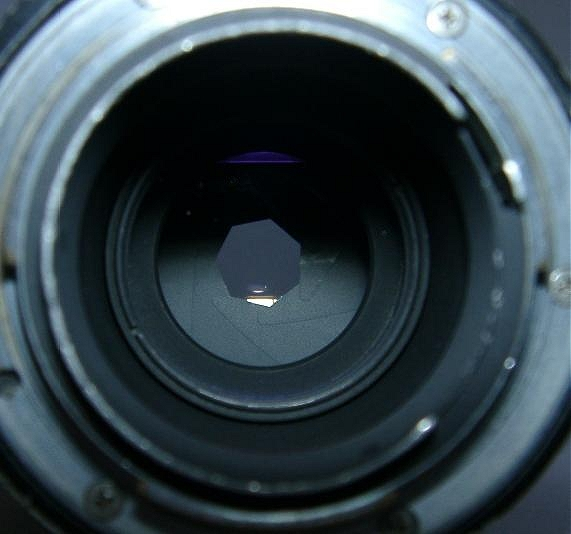
\includegraphics[width=25mm]{aperture}
			\caption{Bländare}
		\end{wrapfigure}
		Bländaren i en kamera är en anordning som reglerar mängden ljus som släpps in kamerahuset. Bländaren och slutartiden samarbetar för att exponera kamerans bildsensor, med rätt mängd ljus. 
		Man kontrollerar att bilden har rätt mängd ljus genom att föra in en list i kameralådan så att en sträckkod är i bild. Bilden skall vara så ljus att sträckkoden inte flyter ihop, 
		och så mörk att texten ändå har hög kontrast mot listen. Eftersom att kameran sitter i en låda påverkas inte bilden så mycket utav omgivningens belysning. 
		Men LED panelens ljus kommer gradvis att bli sämre. Därför är det en god ide att kontrollera detta vid varje uppstart.
		Öppnar man bländaren för mycket kan man få problem med att bilden blir för
		ljus. Det blir då svårt att justera tröskelvärdet. }%vbox

	\vbox{\subsection{Aktivering av larm}\label{subsec:activatealarm}
		\begin{wrapfigure}{R}{3cm}
		  	\vspace{-5mm}
			\centering
			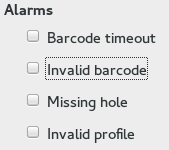
\includegraphics[width=25mm]{alarm_checkboxes}
			\caption{Aktivering larm}\label{fig:alarm_checkboxes}
		\end{wrapfigure}

	  	Man kan aktivera/avaktivera larm manuellt genom att kryssa i/ur rutorna under rubriken Alarms (se bild \ref{fig:alarm_checkboxes}). Larmen finns beskrivna i kapitel \ref{sec:alarms}.
	  	\newline 
	  	\newline 
		De tillgängliga larmen är:

		\vbox{
		\begin{itemize}
			\item Barcode timeout. Se kapitel~\ref{subsec:barcode_timeout}
			\item Invalid barcode. Se kapitel~\ref{subsec:invalid_barcode}
			\item Missing hole. Se kapitel~\ref{subsec:missing_hole}
			\item Invalid profile. Se kapitel~\ref{subsec:invalid_profile}
		\end{itemize}}
	      }%vbox
	
	\vbox{\subsection{Val av sträckkod}
		\begin{wrapfigure}{R}{3cm}
		  	\vspace{-5mm}
			\centering
			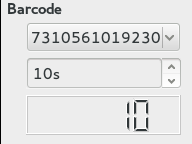
\includegraphics[width=25mm]{barcode_settings}
			\caption{Inställningar sträckkod}
		\end{wrapfigure}
		Under rubriken \textbf{Barcode} hittar man en rullgardinsmeny innehållande förvalda sträckkoder. Om programmet detekterar en annan sträckkod än den som är vald kommer larmet 
		Invalid Barcode (se kapitel \ref{subsec:invalid_barcode}) aktiveras.
		Information om hur man lägger till fler sträckkoder finns i kapitel \ref{subsec:barcode}.\newline
		I stegningsrutan väljer man hur många sekunder som går från det att kameran ser en giltig sträckkod tills dess att den larmar för timeout sträckkod (se kapitel \ref{subsec:barcode_timeout}).\newline
		I LCD displayen under stegningsrutan ser man återstående tid när kameran är startad.
	      }

	\vbox{\subsection{Åtgärder vid uppstart}
	    När maskinen är startad och profilen passerar igenom kameralådan behöver man kontrollera två stycken inställningar. 
	    Det kan vara en bra ide att stänga av alla larm innan man gör dessa inställningar. 
	    Kryssa ur samtliga rutor under rubriken \textbf{Alarms}. Därefter justerar man bländaren och tröskelvärdet.
	    \subsubsection{Checklista uppstart}
		    \vbox{ %Tillåt inte att listan delas upp på två olika sidor
		    \begin{itemize}
		    \item Starta maskinen.
		    \item Kryssa ur samtliga larm. Se kapitel~\ref{subsec:activatealarm}
		    \item Starta kameran.
		    \item Justera bländaren. Se kapitel~\ref{subsec:aperture}
		    \item Justera tröskelvärdet. Se kapitel~\ref{subsubsec:threshold}
		    \item Stoppa kameran.
		    \item Välj vilka larm som skall vara aktiverade. Se kapitel~\ref{subsec:activatealarm}
		    \item Starta kameran.
		    \end{itemize}}
	      }
	    
	\subsection{Åtgärder under körning}
		\subsubsection{Återställning av larm}
			Larmen återställs genom att trycka på den orangea knappen bredvid skärmen på elskåpet.

\section{Larm}\label{sec:alarms}
	Larm indikeras genom ljus och ljudsignal på elskåpet. Information om larmen lagras i en lista under fliken \textbf{Alarms} (bild \ref{fig:alarm_list}).

	\begin{figure}[H]
	  	\centering
		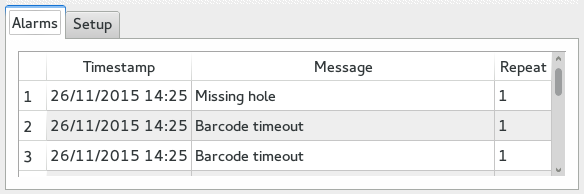
\includegraphics[width=0.7\textwidth]{alarm_list}
		\caption{Larmlista}\label{fig:alarm_list}
	\end{figure}
	\textit{Timestamp} är tidpunkten då larmet först aktiverades. \textit{Message} innehåller information om vilket larm som avses. \textit{Repeat} visar hur många gånger i rad det larmet har aktiverats.

	\subsection{Timeout sträckkod}\label{subsec:barcode_timeout}
		Programmet letar efter en sträckkod i varje bild som kommer från kameran. En timer räknar ner varje sekund.
		När en giltig sträckkod hittas i bilden återställs timern till sitt förinställda värde. Larmet aktiveras när timern räknat ner till 0.

	\subsection{Ogiltlig sträckkod}\label{subsec:invalid_barcode}
		Detta larm aktiveras när en annan sträckkod än den förvalda upptäcks i en bild.

	\subsection{Hål saknas}\label{subsec:missing_hole}
		Aktiveras när programmet upptäcker att det horisontella avståndet mellan två hål avviker från de andra hålavstånden på den raden.
		Falsklarm kan bero på för snäva inställningar gällande hålets rundhet och storlek, eller att tejpen hamnat mitt för ett hål och tröskelvärdet är inställt
		på ett sådant sätt att tejpen blir en del av profilen.

	\subsection{Ogiltlig profil}\label{subsec:invalid_profile}
	Detta larm aktiveras när programmet inte hittar en profil i bilden. Det kan bero på att profilen inte längre matas genom lådan, om det blivit fel på kameran eller om parametern \textit{min\_profile\_area}
	är ställd för högt (se kapitel \ref{subsubsec:min_profile_area}).

\section{Inställningar}
	\subsection{Kamera}
		Kameran har förutom exponeringstiden inställningar gällande ROI eller Region Of Interest. ROI avser den för oss intressanta delen av bilden. 

	    \subsubsection{Exponeringstid}
		  Inom fotografi är exponeringstid den tid slutaren hålls öppen för att låta ljuset träffa bildsensorn i kameran då ett fotografi tas. 
		  Tillsammans med objektivets bländare bestämmer detta hur pass exponerad filmen kommer att bli. 
		  En kort slutartid behöver en större bländaröppning för att undvika underexponering och en lång slutartid kompenseras av en mindre bländaröppning för att undvika överexponering.

	    \subsubsection{ROI x}
		  Start x-kordinat för vår region of interest.

	    \subsubsection{ROI y}
		  Start y-kordinat för vår region of interest.

	    \subsubsection{ROI bredd}
		  Bredden på vår region of interest.

	    \subsubsection{ROI höjd}
		  Höjden på vår region of interest.

	\subsection{Hål}
		När hålen detekterats filtreras de efter area och cirkuläritet. Därefter sorteras de in i rader, sedan sorteras de från vänster till höger.
		Efter att de sorterats mäts centrum-centrum avstånden mellan hålen på respektive rad. Medelavståndet räknas fram och därefter söker programmet igenom
		centrum-centrum avstånden igen och jämför mot medelavståndet. \newline\newline
		Cirkuläriteten räknas ut genom att mäta avståndet från hålets mest vänstra pixel till den längst till höger. Sedan räknar man ut arean på hålet $a_h$ och 
		arean på en perfekt cirkel med en diameter motsvarande hålets maximala bredd $a_p$. Cirkuläriteten räknas sedan ut med $\frac{a_p}{a_h}$. En perfekt cirkel har då en cirkuläritet på 1.0.

	  \subsubsection{Maximal avvikelse Y}
	  	Parametern \textit{max\_y\_dev} representerar hur många gånger medelavståndet i Y koordinat ett hål måste avvika från medel för att det skall
		räknas som en ny rad.

	  \subsubsection{Minimal cirkularitet}
	    	Parametern \textit{min\_circularity} representerar den lägsta accepterade cirkuläriteten ett hål får ha. Samtliga hål med lägre cirkuläritet filtreras bort.
	  	
	  \subsubsection{Maximal cirkularitet}
	  	Parametern \textit{max\_circularity} representerar den högsta accepterade cirkuläriteten ett hål får ha. Samtliga hål med en högre cirkuläritet filtreras bort.

	\subsection{Allmänt}
	  \vbox{\subsubsection{Tröskelvärde}\label{subsubsec:threshold}
		\begin{wrapfigure}{R}{3cm}
			\centering
			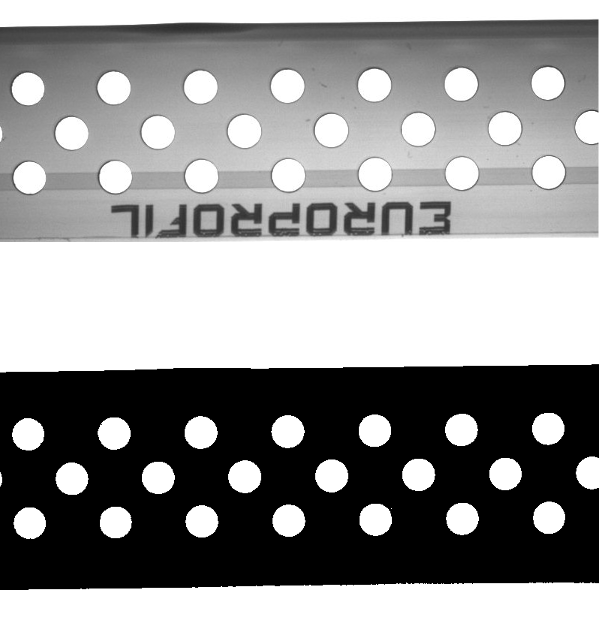
\includegraphics[width=25mm]{threshold}
			\caption{Tröskel}
			\vspace{5mm}
			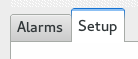
\includegraphics[width=25mm]{tab_setup}
			\caption{Flik setup}
		\end{wrapfigure}
		Kameran som fotograferar listen tar bilder i gråskala. Man kan tänka på en sådan här bild som ett rutnät av färgvärden från 0 till 255 där 0 är svart och 255 är vit. 
		Alla värden där emellan är olika nyanser av grått. 
		Att ta ett tröskelvärde på en bild innebär att man väljer en nivå mellan 0-255. Alla pixlar som är < nivån blir svarta och alla som är > nivån blir vita. 
		Målet med detta är att få ut en bild som endast innehåller en enfärgad representation av vinkelprofilen. Detta för att möjliggöra att man kan detektera och mäta hålen i profilen.
		Det är en bra ide att börja med ett lågt värde och gradvis öka tills man har en solid bild av profilen där hålen syns tydligt utan att smälta ihop. \newline
		Tröskelvärdet justeras genom att välja fliken Setup och dra spaken märkt Threshold i sidled alternativt via Settings->General.
		Om man fortfarande ser fläckar i profilen när man ställt upp tröskelvärdet
		till sitt max värde betyder det att bländaren släpper in för mycket ljus.
		Justera då bländaren för att få en mörkare bild (se kapitel
		\ref{subsec:aperture}). }

	      \subsubsection{Minimal profilarea}\label{subsubsec:min_profile_area}
	  	Efter det att programmet tagit ett tröskelvärde på bilden försöker det urskilja vilken del av bilden som är vår vinkelprofil. 
		Detta går till så att bilden delas upp i områden med sammanhängande pixlar och det största området anses vara profilen. Parametern \textit{min\_profile\_area} representerar det
		minsta antalet sammanhängande pixlar som skall vara med i den uttagningsprocessen. Här rekommenderas ett så högt värde som möjligt.

	  \subsubsection{Minimal hålarea}
	  	När profilen är hittad börjar processen med att hitta hålen. Parametern \textit{min\_hole\_area} representerar det minsta antalet pixlar 
	  	som kan utgöra ett hål.
		Alla hål med en mindre area än detta ignoreras.

	\subsection{Sträckkod}\label{subsec:barcode}
	  \subsubsection{Timeout}
	  	Tiden från det att programmet detekterat en giltig sträckkod och det att larmet Barcode timeout aktiveras. Detta värde ändras med fördel i huvudprogrammets stegruta.

	  \subsubsection{Giltliga sträckkoder}
	  	Detta är listan med giltliga sträckkoder. En sträckkod får endast innehålla siffror. Sträckkoderna separeras med ett radbyte.

\section{Underhåll}
	LED panelen i kameralådan behöver hållas ren för att undvika felläsning och falsklarm.

\end{document}
